\documentclass[border=10pt]{standalone}
\usepackage{tikz}

\begin{document}

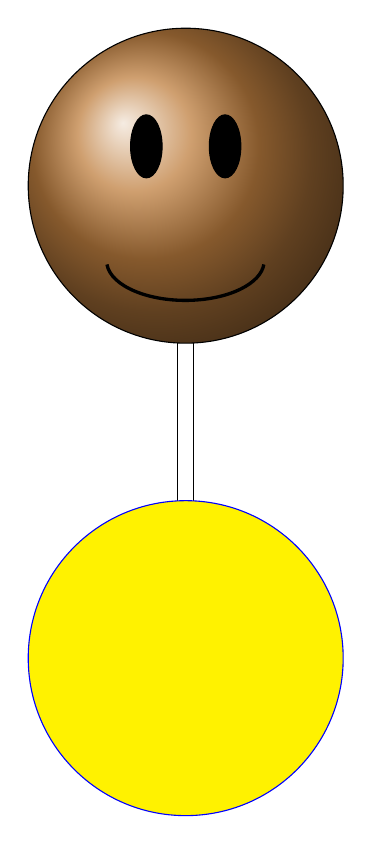
\begin{tikzpicture}
    \coordinate (baseupperdrawing) at (0,3);
    \coordinate (basebottomdrawing) at (0,-3);
    \begin{scope}[shift={(baseupperdrawing)}]
    \draw[shading=ball, ball color=brown] (0,0) circle [radius=2];%ball is a predefined shading
    \draw[fill=black] (-0.5,0.5,0) ellipse [x radius=0.2, y radius=0.4];
    \draw[fill=black] (0.5,0.5,0) ellipse [x radius=0.2, y radius=0.4];
    \draw[very thick] (-1,-1) arc [start angle=185, end angle=355, x radius=1, y radius=0.5];
        % \draw (0,-1) ellipse [x radius=1, y radius=0.5][thick, color=blue] ;%ellips arc is begint op aangegeven coordinaat, tis niet dat de ellips wrvn de arc komt daarop gecenterd is
    \end{scope}
        \draw (-0.1,1)--(-0.1,-1);
        \draw (0.1,1)--(0.1,-1);
    \begin{scope}[shift={(basebottomdrawing)}]
        \draw (0,0) circle [radius=2][blue,fill=yellow];


    \end{scope}



        
\end{tikzpicture}
\end{document}